\documentclass[10pt,a4paper]{article}
\usepackage[a4paper, top=2cm, bottom=1.5cm, left=1.5cm, right=1.5cm]{geometry} % Задать размеры полей.
\usepackage[warn]{mathtext} % Русские символы в формулах. Нужно писать до пакета babel. Указывает, что в формулах используются символы кириллицы, которые по умолчанию печатаются прямым шрифтом.
\usepackage[T2A]{fontenc}
\usepackage[utf8]{inputenc}
\usepackage[russian]{babel}
\usepackage{amsmath}
\usepackage{amssymb}
\usepackage{graphicx}
%\usepackage{floatrow}
\usepackage{booktabs}
\usepackage{wrapfig}
\usepackage{fancyhdr}
\usepackage{multicol}
\usepackage{xcolor}

\usepackage{float}
\usepackage{multirow}

\usepackage{subfigure}

% Объявляем новую команду для переноса строки внутри ячейки таблицы
\newcommand{\specialcell}[2][c]{%
	\begin{tabular}[#1]{@{}c@{}}#2\end{tabular}}

\newcommand{\figref}[1]{(См. рис. \ref{#1})}
\newcommand{\secref}[1]{(См. раздел. \ref{#1})}

\newcommand{\angstrom}{\text{\normalfont\AA}}
\newcommand{\e}[1]{\text{$\cdot10^{#1}$}}
\newcommand{\m}{\; м}
\newcommand{\mm}{\; мм}
\newcommand{\um}{\; мкм}
\newcommand{\A}{\; А}
\newcommand{\V}{\; В}
\newcommand{\uV}{\; мкВ}
\newcommand{\cels}{\; ^\circ С}

\pagestyle{fancy}
\fancyhead{}
\fancyhead[L]{\small Дедков Д.А., Маслов А.С., Измерение абсолютной активности препарата ${}^{60}Co$ методом $\gamma-\gamma$ совпадений. МФТИ, 2023 г.}
\fancyhead[R]{}
\fancyfoot[C]{\thepage}

\renewcommand{\cot}{\text{ctg}}

\author{\normalsize Маслов Артём, Дедков Денис \\
	\normalsize группа Б01-108а \\
	\normalsize 30.10.2023}
\date{}

\title{
	\Large Измерение абсолютной активности препарата ${}^{60}Co$ методом $\gamma-\gamma$ совпадений. \\ 
}

\begin{document}
\maketitle
	
	\subsection*{Цель и задачи работы:}
	\begin{enumerate}
		\item Определить абсолютную активность радиоактивного препарата ${}^{60}Co$ с использованием каскадного перехода $\gamma-$квантов при его распаде.
	\end{enumerate}
	
	\subsection*{Описание экспериментальной установки}
	
	Схема экспериментальной установки приведена на рисунке \ref{img:exp_scheme}:
	\begin{figure}[H]
		\centering
		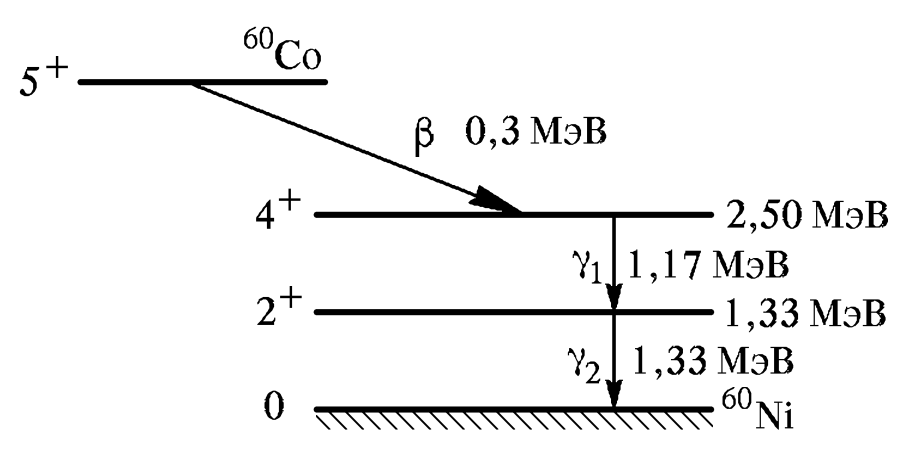
\includegraphics[width=0.45\textwidth]{images/radio_scheme.png}
		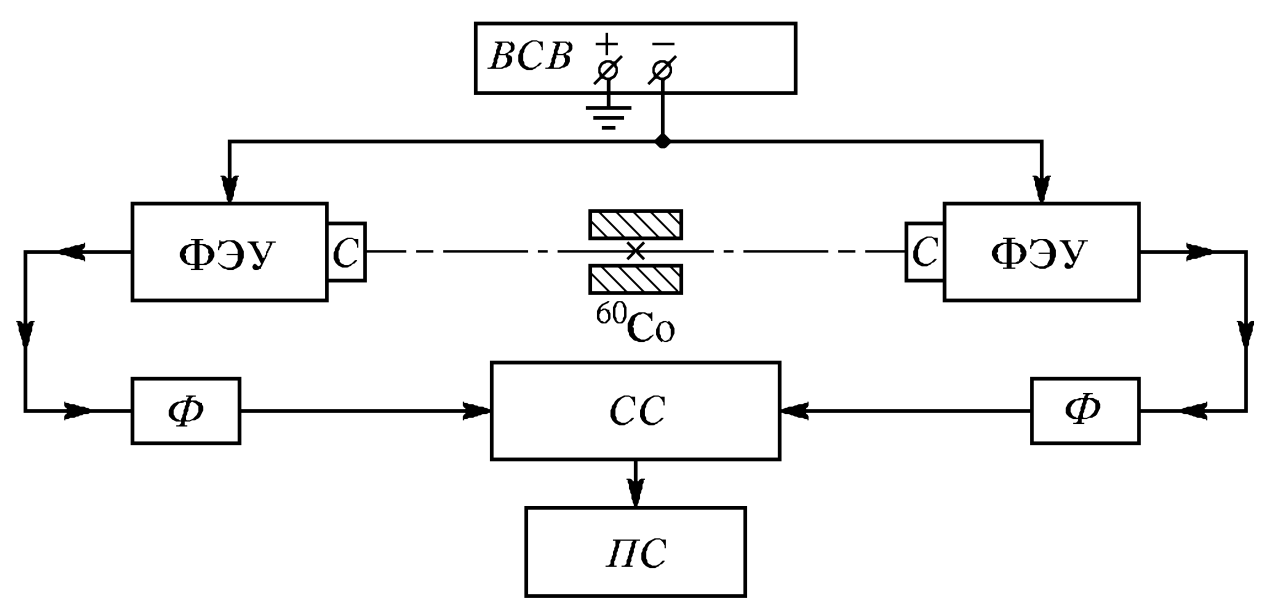
\includegraphics[width=0.45\textwidth]{images/exp_scheme.png}
		\caption{Слева схема каскадного $\gamma$-распада. Справа схема экспериментальной установки.}
		\label{img:exp_scheme}
	\end{figure}

	Гамма-кванты от источника ${}^{60}Co$ регистрируются двумя сцинтилляционными счётчиками, каждый из которых состоит из кристалла $NaI(Tl)$ и фотоэлектронного умножителя (ФЭУ). При поглощении $\gamma-$кванта кристаллом возникает световая вспышка, которая преобразуется с помощью ФЭУ в электрический импульс, передаваемый через формирователь импульсов на схему совпадений СС и регистрируемый пересчётчным прибором ПС. Фотоэлектронные умножители питаются от высоковольтного стабилизированного выпрямителя.
	
	\subsection*{Оборудование и приборы}
		
	\begin{enumerate}
		\item Лабораторная установка для исследования абсолютной активности кобальта-60 $ЛУ-4.3-2$. Заводской номер №1513. Инвентарный номер №410134174169.
		
		\item Блоки детектирования сцинтилляционные БДЕГ-40.
		  
	 	\begin{enumerate}
	 		\item Заводской номер №2907. Инвентарный номер №410134174169. Инвентарный номер №4008.
	 		
	 		\item Заводской номер №2908. Инвентарный номер №4026.
	 		
	 		\item Пересчётное устройство. Инвентарный номер №410134125664.
	 	\end{enumerate}
	\end{enumerate}
	
	\subsection*{Первичные экспериментальные данные}
		
	Первичные экспериментальные данные приведены в таблицах 1-3.
	
	\begin{tabular}[t]{c}
		Таблица 1. Измерение фона. \\
		\input{gen/tab-noise.tex} \\
		\begin{tabular}[t]{l}
			Индексы 1 и 2 указывают на детектор, которым производились измерения. $t$ -- время измерения,
			$N$ -- полное \\количество импульсов, $n$ -- количество импульсов за секунду,
			$\sigma_{n}$ -- погрешность измерения $n$.
		\end{tabular}
	\end{tabular}
	
	\begin{tabular}[t]{c}
		Таблица 2. Измерение в режиме совпадений. \\
		\input{gen/tab-overlap.tex} \\
		\begin{tabular}[t]{l}
			$\tau$ -- время регистрации совпадения, $t$ -- время измерения,
			$N$ -- полное количество импульсов, $n$ -- количество \\импульсов за секунду,
			$\sigma_n$ -- погрешность измерения $n$.
		\end{tabular}
		\end{tabular}

	\begin{tabular}[t]{c}
		Таблица 3. Измерение каждым детектором отдельно. \\
		\input{gen/tab-separate.tex} \\
		Индексы 1 и 2 указывают на детектор, которым производились \\
		\begin{tabular}[t]{l}
			Индексы 1 и 2 указывают на детектор, которым производились измерения. $t$ -- время измерения,
			$N$ -- полное \\количество импульсов, $n$ -- количество импульсов за секунду,
			$\sigma_{n}$ -- погрешность измерения $n$.
		\end{tabular}
	\end{tabular}
	
	Время измерялось цифровым прибором, погрешность измерения времени $\sigma_t$ можно оценить его тактовой частотой, которая для современных микроконтроллеров обычно составляет $\sim МГц$. Относительная погрешность $\varepsilon \sim 10^{-6}$ пренебрежимо мала. Погрешность измерения импульсов $N$ определяется согласно распределению Пуассона как $\sigma_N = \sqrt{N}$. Погрешность вычисления количества импульсов за единицу времени оценивается по формуле $\varepsilon_n = \varepsilon_N \Rightarrow \sigma_n = n \cdot \sigma_N / N$, так как $n = N/t$. Погрешность задания времени регистрации импульса $\tau$ не известна, так как не известна внутренняя схема пересчётного прибора.
	
	\subsection*{Обработка экспериментальных данных}
	
	Определим среднее значение радиоактивного фона, регистрируемого детекторами:\\
	$n_{ф1} = 33.9 \pm 0.3 \; имп/сек$\\
	$n_{ф2} = 27.1 \pm 0.3 \; имп/сек$\\
	Так как погрешность отдельного измерения связано со случайным распределением распавшихся атомов, то погрешность среднего оценим по формуле $\sigma_{ср} = \sigma_{отд} / \sqrt{k}$, где $k$ -- количество измерений.
	
	Определим средние значения количества зарегистрированных импульсов счётчиками за единицу времени (сигнал + фон):\\
	$n_{1} = 2738 \pm 3$\\
	$n_{2} = 1013 \pm 2$\\
	Так как погрешность отдельного измерения связано со случайным распределением распавшихся атомов, то погрешность среднего оценим по формуле $\sigma_{ср} = \sigma_{отд} / \sqrt{k}$, где $k$ -- количество измерений.
	
	Определим средние значения количества распавшихся атомов ${}^{60}Co$, зарегистрированных счётчиками за единицу времени:\\
	$n_{р1} = n_{1} - n_{ф1} = 2704 \pm 3$\\
	$n_{р2} = n_{2} - n_{ф2} = 987  \pm 2$\\
	Погрешность оценим по формуле $\sigma_{n} = \sqrt{\sigma_{n_{с+ф}}^2 + \sigma_{n_ф}^2} \approx \sigma_{n_{с+ф}}^2$.
	
	Число случайных совпадений определим по формуле:
	$$n_{сл} = 2 \tau n_{1} n_{2}$$
	Погрешность оценим по следующей формуле:
	$$\sigma_{n_{сл}} = n_{сл} \cdot \sqrt{ \left(\frac{\sigma_{n_1}}{n_1}\right)^2 + \left(\frac{\sigma_{n_2}}{n_2}\right)^2 }$$
	
	Полное число совпадений вычисляется по формуле:
	$$
	n_{совп} = n - n_{сл}
	$$
	Погрешность оценим как
	$$
	\sigma_{n_{совп}} = \sqrt{n^2 + n_{сл}^2}
	$$
	
	Абсолютная активность источника равна
	$$
	N_0 = 1.08 \frac{n_{р1} n_{р2}}{2 n_{совп}}
	$$,
	где $1.08$ -- поправка, связанная с не идеальным разлётом гамма-квантов под углом $180^\circ$.
	
	Результаты вычислений сведём в таблицу:\\
	\begin{tabular}{ccccccc}
		\hline
		$\tau, \; мкс$ & $n_{сл}, имп$ & $\sigma_{n_{сл}}, имп$ & $n_{совп}, имп$ & $\sigma_{n_{совп}}, имп$ & $N_0, \; мкКи$ & $\sigma_{N_0}, \; мкКи$ \\
		\hline
		0.2 & 1.111 & 0.003 & 0.86 & 0.06 & 45 & 3 \\
		0.5 & 2.776 & 0.007 & 0.70 & 0.09 & 55 & 7 \\
		1.0 & 5.553 & 0.013 & -0.33 & 0.15 & -117 & 52 \\ 
		\hline
	\end{tabular}

	Причину отрицательного результата для $\tau = 1.0 \; мкс$ установить не удалось. Скорее всего это связано с малым временем наблюдения числа импульсов в режиме совпадения.

	Построим график зависимости $N_0(\tau)$.
	\begin{figure}
		\centering
		\includegraphics[width=0.5\textwidth]{gen/n0_tau.png}
		\caption{График зависимости $N_0(\tau)$. Точку $\tau=1 \; мкс$ отбрасываем.}
	\end{figure}

	Определим среднее значение активности препарата:\\
	$N_0 = 50 \pm 4 \; мкКи$.
	
	\subsection*{Обсуждение результатов и выводы}
	
	В работе было измерено среднее значение активности препарата ${}^{60} Co$ методом гамма-гамма совпадений:\\
	$N_0 = 50 \pm 4 \; мкКи$.
		
\end{document}